\documentclass[a4paper,11pt]{article}
%\documentclass[a4paper,10pt]{scrartcl}

\usepackage[utf8]{inputenc}
\usepackage[a4paper,
            bindingoffset=0.2in,
            left=1in,
            right=1in,
            top=1in,
            bottom=1in,
            footskip=.25in]{geometry}
\usepackage{graphicx}
\usepackage{float}
\usepackage{tabu}
\usepackage{xcolor}
\usepackage{fancyhdr}
\usepackage{hyperref}
\hypersetup{
    colorlinks=true,
    linkcolor=blue,
    filecolor=magenta,      
    urlcolor=cyan
    }
\usepackage{tocloft}
\renewcommand{\cftsecleader}{\cftdotfill{\cftdotsep}}
\usepackage{titling}
\renewcommand\maketitlehooka{\null\mbox{}\vfill}
\renewcommand\maketitlehookd{\vfill\null}
\usepackage{parskip}
\graphicspath{{../figures/}}

\title{Using Autoencoders to Detect Errors in Telemetry Events}
\author{Andrew Younger}
\date{\today}

\begin{document}
\pagenumbering{gobble}
\begin{titlingpage}
 \maketitle
\end{titlingpage}
\newpage
\pagenumbering{roman}
\tableofcontents
\newpage
\pagenumbering{arabic}
\section{Introduction}
Telemetry events are essential for accurate reporting on player activity and progress for modern games. They allow the analytics team to dive deeply into topics and analyze important questions from stakeholders in the project. These events can be quite expansive, detailing anything from how a player kills an enemy to what cosmetics a player applies to their character to how quickly players are able to complete the game.
\par
During the development cycle of a game there are frequent code changes which can affect telemetry frequently both accidentally and by design. QC teams work diligently in order to keep up with testing events as they are created but changes that affect older events often produce bugs which impact reporting done by the analytics team for playtests. In addition, telemetry events can be quite large and have many attributes with many different possibilities. A player.kill event, for example, where there are 50 weapons and 50 enemy types tracked yiels 2500 possibilities in just two columns. This further exacerbates the issues that the QC teams face when trying to catch every erroneous scenario that occurs inside telemetry events leading to the questions of: ``How do we determine when an event has bugs?'' and ``How do we know when QC teams should retest old events?''.
\par
An immediate proposition to answer these questions is to use some form of automated bug detection. There are two methods of bug detection which could be helpful for QC teams to track down and deal with bugs: checking for some sort of spike in event frequency (if events start transmitting too often or stop transmitting then there may be an issue with the event's trigger mechanism) and statistsically determining if event attribute A is supposed to match with event attribute B. This report outlines a process for the second method by using an autoencoder to learn the possibility space of an event.
\subsection{Autoencoders}
Autoencoders are type of neural network that fall into the \textit{encoder-decoder} family of neural networks. The general process for an autoencoder is shown in Figure \ref{autoencoder_general}. The encoding section of an autoencoder learns to ``compress'' the data down into a smaller dimension so that the decoding section of the autoencoder can attempt to recreate the original data from this low-level representation of the data. Autoencoders are used for several purposes including: image denoising, facial recognition, and, importantly for finding bugs, anomaly detection.
\begin{figure}[H]
\centering
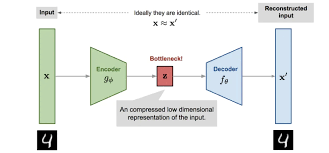
\includegraphics[width=.8\textwidth]{autoencoder_general.png}
\caption{The general layout of an autoencoder network. The network works by learning efficient compression to a low dimension and then reconstructing the data as closely as possible \cite{patil}.}
\label{autoencoder_general}
\end{figure}
Using an autoencoder to detect anomalies in data is very straightforward.

\newpage
\begin{thebibliography}{100}
\bibitem{patil} Akshay Gadi Patil, Omri Ben-Eliezer, Or Perel, and Hadar Averbuch-Elor, ``Recursive Autoencoders for Document Layout Generation'' {\tt arXiv:1909.00302v4 [cs.CV]}
\end{thebibliography}


\end{document}
